\documentclass{jfp}

\usepackage{ifpdf}
\usepackage{ifthen}
\usepackage{subfigure}
\usepackage{epsfig}

\usepackage{textcomp}
\usepackage{mathtools}
\usepackage{subfigure}
\usepackage{epsfig}
\usepackage{amssymb}
%\usepackage{amsthm}
\usepackage{enumerate}


\title{\LARGE \bf
A simpler approach to waterfall
}
\author{Chris Nicholls, Irina Voiculescu and Stuart Golodetz
}
%\institute{Oxford University Computing Laboratory}

\begin{document}

\maketitle

\begin{abstract}
It is useful to be able to identify particular features in a set of
images automatically. One application is in the treatment of cancer,
where algorithms can be used to aid the detection and classification
of organ and tumour tissue. This is the main motivation for this
project, although the algorithm presented is a generic one, with many
applications. 
In this paper we present a refinement of the {\em waterfall\/}
algorithm which simplifies the process and improves efficiency
compared to existing implementations. 
We also show how the algorithm can be written as a single recursive
pass of the MST and how it can be written in a pure functional style.


\end{abstract}

\section{Introduction}

This work has been motivated by the need to {\em segment\/} greyscale
images originating from computerised tomography (CT) scanners. That
is, we would like to fit contours around organ tissue featured in each
image. A pair of algorithms called the {\em watershed\/} and {\em
waterfall\/} algorithms -- proposed for the generic segmentation
  problem -- have been shown to be effective for the purpose of CT
  imaging~\cite{golodetz}, although other approaches exist. This paper
  presents a new, simplified, implementation of the {\em waterfall\/}
  algorithm.

\section{Conventional imperative approach to waterfall}

The {\em watershed\/} algorithm, introduced by Beucher and
Lantuejoul~\cite{beucher79}, produces a segmentation of an image,
grouping together regions of pixels deemed to be similar. Usually,
`similar' refers to similarity in the greyscale values, though other
approaches are possible. A typical problem of the watershed algorithm
is that it over-segments images significantly, leading to far more
regions than can be handled sensibly, as illustrated in
Figure~\ref{fig:oversegmented}.

%---
%---
\begin{figure}
\centering
\ifpdf
        \subfigure{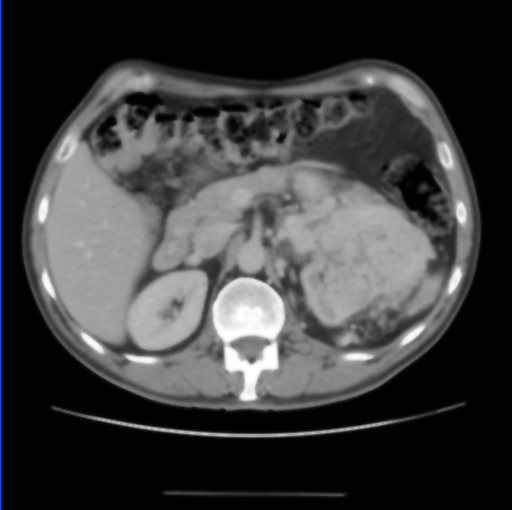
\epsfig{file=image0.png, width=.240\linewidth}}%
        \hspace{1mm}%
        \subfigure{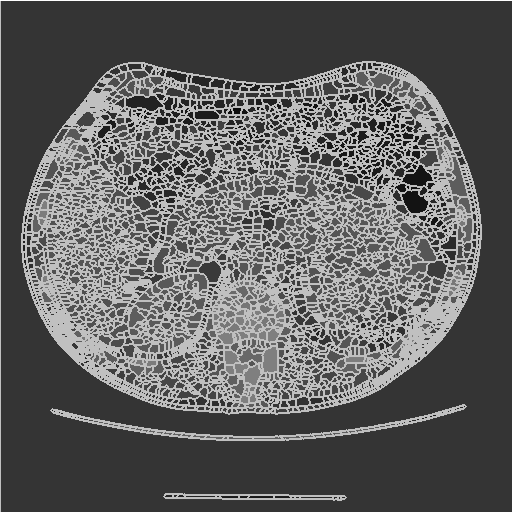
\epsfig{file=image5.png, width=.240\linewidth}}%
\else
        % TODO
\fi
\caption{Example of over-segmentation, output by applying the watershed
  algorithm to an axial slice of a CT volume. The individual regions
  are small and do not correspond to any anatomic features.}
\label{fig:oversegmented}
\end{figure}
%---
%\vspace{-5mm}
% 

The {\em waterfall\/} algorithm~\cite{beucher94,marcotegui} is an
iterative process which can extract further structure from an initial
watershed segmentation. The waterfall yields a partition forest
hierarchy, which is a comprehensive data structure which can
subsequently be used for feature identification.
Figure~\ref{fig:waterfall} illustrates the various layers that result
from applying the waterfall algorithm to the segmentation shown in
Figure~\ref{fig:oversegmented}.  Each iteration of the algorithm
yields a higher-level grouping of the regions in the previous layer.
%\vspace{-5mm}
%---
\begin{figure}
\centering
\ifpdf
%        \subfigure{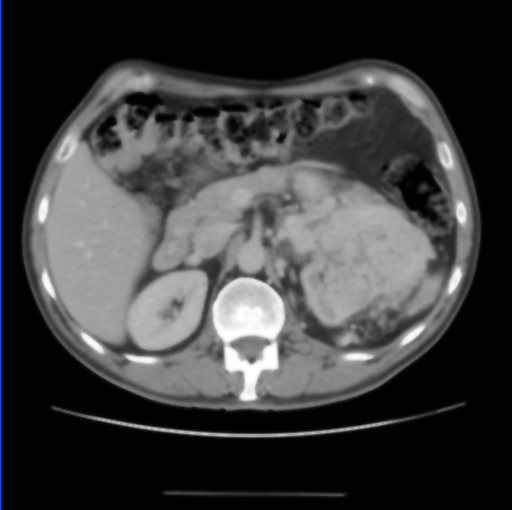
\epsfig{file=image0.png, height=.175\linewidth}}%
%        \hspace{4mm}%
%        \subfigure{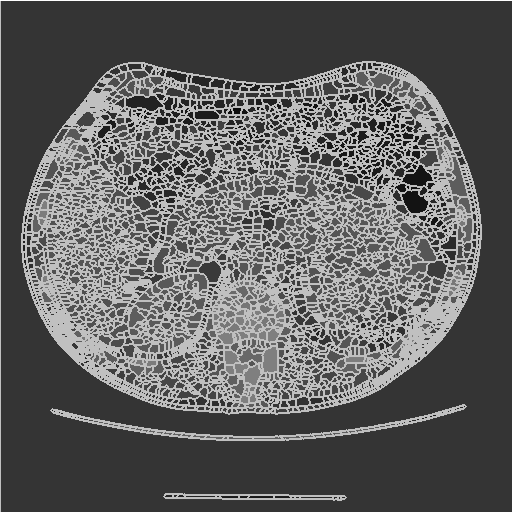
\epsfig{file=image5.png, width=.240\linewidth}}%
%        \hspace{1mm}%
        \subfigure{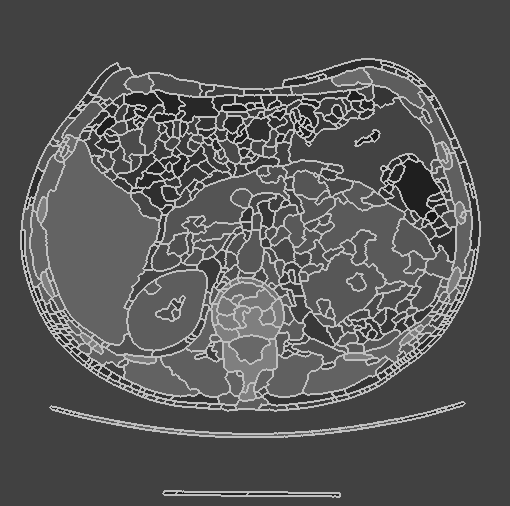
\epsfig{file=image4.png, width=.260\linewidth}}%
        \hspace{1mm}%
        \subfigure{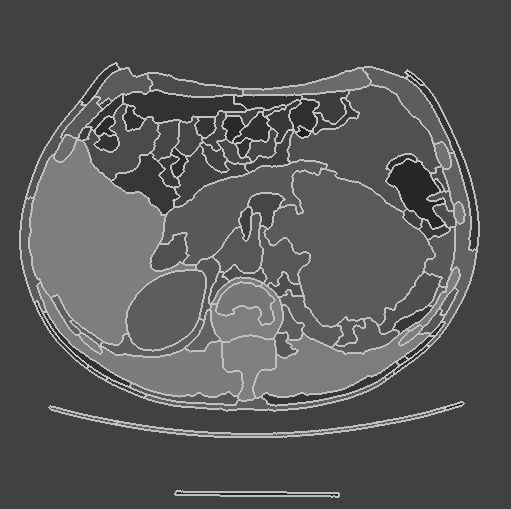
\epsfig{file=image2.png, width=.260\linewidth}}%
        \hspace{1mm}%
        \subfigure{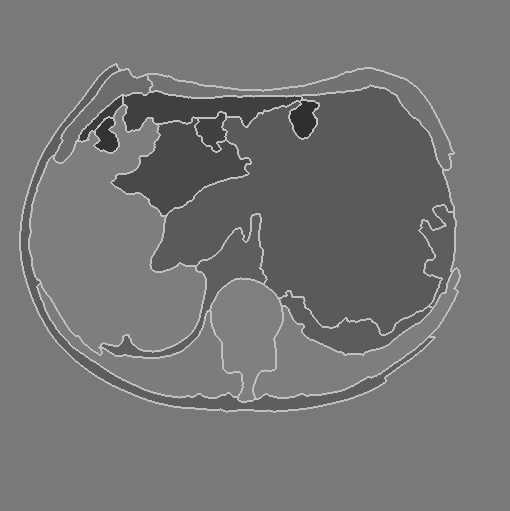
\epsfig{file=image1.png, width=.260\linewidth}}%
\else
        % TODO
\fi
\caption{Hierarchy of segmentations produced by applying the waterfall
  algorithm to the output of the watershed illustrated in
  Figure~\ref{fig:oversegmented}, showing regions merging successively
  (left to right).}
\label{fig:waterfall}
\end{figure}
%---

Both the watershed and the waterfall algorithms are based on a
geographical metaphor. The image is regarded as a landscape, with each
grey value at representing the height of the terrain at given $(x,y)$
coordinates.
% being proportional to the terrain height.
%
The valleys are
in the darker areas, whereas the lighter areas are regarded as peaks.

The waterfall algorithm can then be imagined
as a flooding process. The water falls into (low) catchment basins and
gradually fills them up to the nearest boundaries, sometimes spilling
into adjacent regions. This process continues until the whole image
becomes a single basin. The intermediate stages of the process can be
regarded as intermediate segmentations of the image, with each basin
representing a region.

An imperative implementation of this algorithm, proposed by Marcotegui
and Beucher~\cite{marcotegui}, involves the construction of a Minimum
Spanning Tree (MST) and the gradual elision of some of its edges.  Its
nodes are initially the regions of the watershed output and its edges
are the lowest pass points on the boundaries between these regions;
the nodes and edges in subsequent layers are derived from these
initial ones through a merging process. (As an aside, it is worth
noting that the algorithm allows for the MST to be consumed starting
at any of its nodes.)

A regional minimum edge of any graph $G$ (and hence also of an MST) is
part of a connected subgraph of $G$ whose edges have the same weight
as each other, and whose adjacent edges in $G$ have strictly higher
weights. The waterfall algorithm relies heavily on finding these
regional minimum edges, eliding them and rebuilding the MST -- a
process which not only requires careful implementation of the MST but,
crucially, can be relatively complex and hard to implement.


\section{Functional approach to waterfall}


We present a refinement of the {\em waterfall\/} algorithm which
simplifies the process and improves efficiency compared to existing
implementations. It is based on a recursive-tree data structure and a
recursive relation on the nodes rather than the conventional iterative
transformations.

We also show how the algorithm can be written as a single recursive
pass of the MST and how it can be written in a pure functional style.


\subsection{Data structure}

The tree structure is defined as

\begin{verbatim}
data Tree a = Node a [Edge a]
data Edge a = Edge Int (Tree a)
\end{verbatim}

That is a tree rooted at a {\tt Node}; a {\tt Node} is a region and a
list of weighted edges to its children. Whilst this would be
sufficient to define a tree structure, we find during the course of
the algorithm it is useful to be able to refer to the same tree as a
collection of {\tt Edge} of particular weights.



The waterfall algorithm relies on identifying the edge of minimum
weight which is adjacent to each node, and eliding it. This amounts to
merging the two regions corresponding to the two node extremities of
that edge.  (For brevity we will refer to such edges as `the minimum
edge {\em of\/} that node'.) Figure~\ref{fig:merging} illustrates an
example of merging.

\begin{figure}
\centering
\ifpdf
        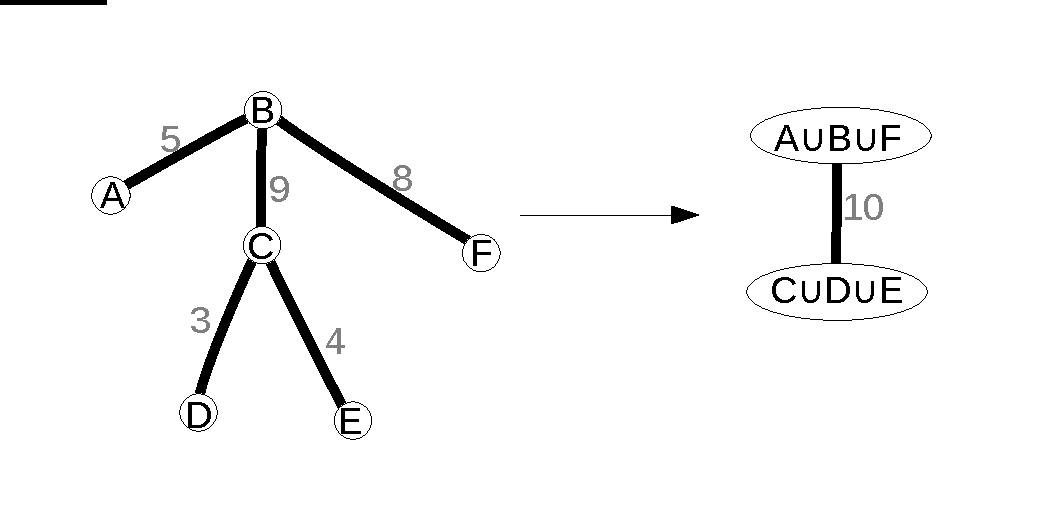
\epsfig{file=waterfallexampleofsetunion.pdf, width=.7\linewidth}%
\else
        % TODO
\fi
\caption{Merging nodes}
\label{fig:merging}
\end{figure}

Since the waterfall algorithm works by merging edges, we will need a
{\em merge} operation on each region of the graph. To do this we
define a type {\tt class Mergeable}.

\begin{verbatim}
class Mergeable a where
  union :: a -> a -> a
  unions :: [a] -> a
  unions = foldl union empty
  empty :: a
  empty = unions []
\end{verbatim}


\subsection{Algorithm outline}


Working recursively down the tree, there are four cases to consider
for an edge $e$ between a parent node $p$ and a child node $c$.
\begin{enumerate}[I]
\item e is     the minimum edge of p and not the minimum edge of c
\item e is     the minimum edge of p and     the minimum edge of c
\item e is not the minimum edge of p and not the minimum edge of c
\item e is not the minimum edge of p and     the minimum edge of c
\end{enumerate}


This is illustrated with an example in Figure~\ref{fig:cases}.

\begin{figure}
\centering
\ifpdf
        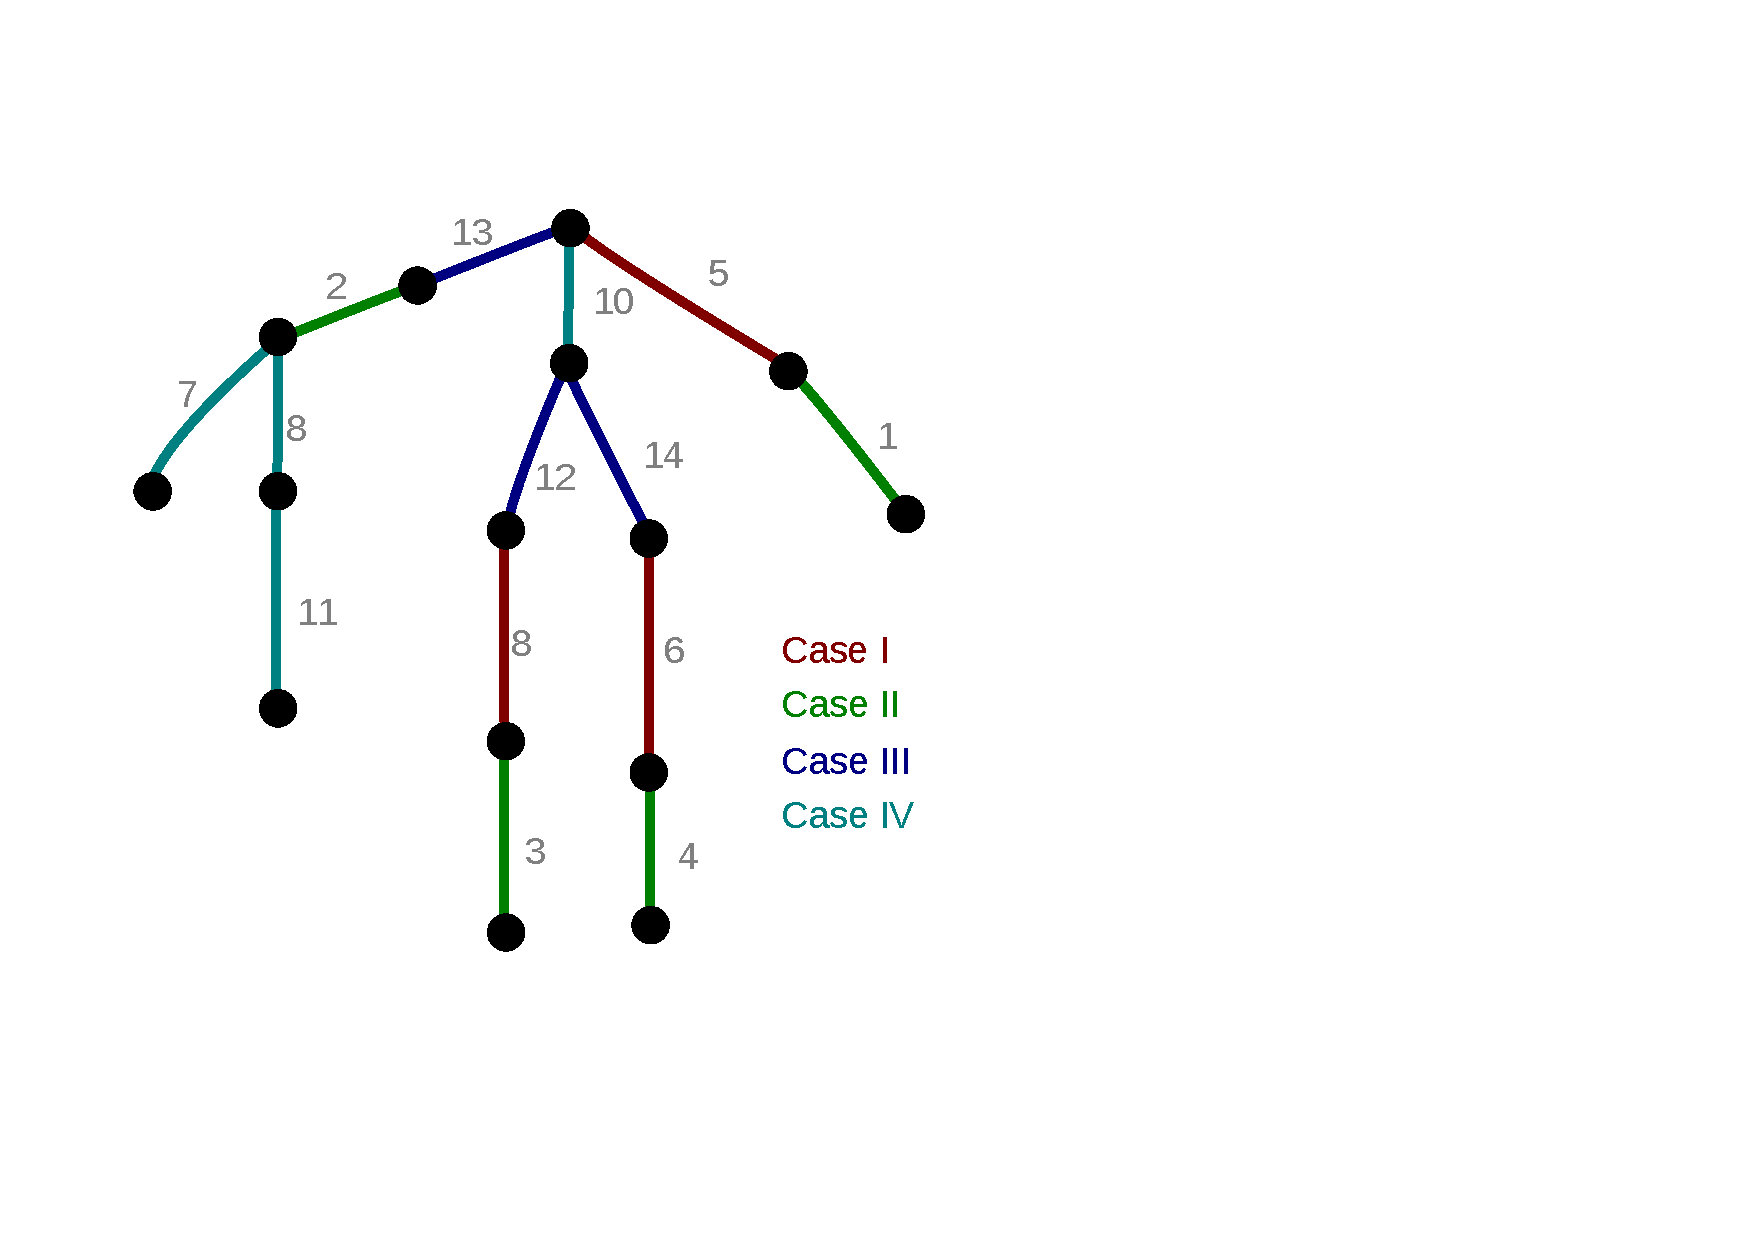
\epsfig{file=treeexamplewithcases.pdf, width=.7\linewidth}%
\else
        % TODO
\fi
\caption{Example of tree with cases}
\label{fig:cases}
\end{figure}


Some things to note:
\begin{enumerate}

\item Precisely one edge from each node will satisfy Case~I or case
  2. All other nodes must be an instance of Case~III or Case~IV.

\item If $e$ satisfies Case~II or Case~IV then we have identified the
  minimum edge of $c$ already so none of $c$'s children can satisfy
  Cases~I or II.

\item For Cases I, II and IV node $p$ and $c$ will be merged and only
  in Case~III will they remain unmerged.

\end{enumerate}

For Cases~I, II and IV node $p$ and $c$ will be merged and only in Case~III
will they remain unmerged and is thus the simplest case to manage.  We
can simply make a recursive call on $c$ having eliminated one of its
children.

We also define a labelled tree that identifies each edge with one of
the cases above.

\begin{verbatim}
data LTree a = LNode a [LEdge a]
data LEdge a = LEdge Label Int (Tree a)
data Label = Case1 | Case2 | Case3 | Case4
\end{verbatim}

The waterfall algorithm will then consist of a pair of functions

\begin{verbatim}
mark  :: Mergeable a => Tree a -> LTree a
elide :: Mergeable a => LTree a -> Tree a
\end{verbatim}

The function elide is simple to define, it walks the tree and merges
each pair of nodes not joined by a Case3 edge because of Lemma 3.

\begin{verbatim}
elide (LNode a []) = Node a []
elide (LNode a ((LEdge l w child):children))  = case l of
    Case3 -> addChild w child' r
    _     -> mergeNodes child' r
    where
      r = elide (LNode a children)
      child' = elide child

addChild :: Int -> Tree a -> Tree a -> Tree a
addChild w child (Node a children) = 
                      Node a ((Edge w child):children)

mergeNodes :: Mergeable a => Tree a -> Tree a -> Tree a
mergeNodes (Node r1 cs1) (Node r2 cs2) = 
                      Node (union r1 r2) (union cs1 cs2)
\end{verbatim}

It now remains only to define the function {\tt mark}. This function
starts at the root of an unlabelled tree and walks through, labelling
each edge. The only edges of the root are its children, so we know the
minimum edge of the root is its smallest child. By Lemma 1, we know
that the minimum child will satisfy either Case~I or Case~II and the
other nodes will satisfy either Case~III or Case~IV.

\begin{verbatim}

mark (Node a []) = LNode a []
mark (Node r cs) = LNode r (case1and2 minChild : map case3and4 cs')
  where
   (minChild,cs') = findMinChild cs


findMinChild :: [Edge a] -> (Edge a,[Edge a])
findMinChild [] = undefined
findMinChild [x]  = (x,[])
findMinChild (x:xs)
   | y < x = (y,x:ys)
   | otherwise = (x,y:ys)
   where (y,ys) = findMinChild xs
\end{verbatim}

Given an edge $e = Edge w t$ that we know to satisfy either Case~I or Case~II, it if fairly easy to tell which sincr $w$ is the smallest edge from t if and only if each edge to a child of t has weight larger than w (or t has no children).
If $s$ is a Case~II edge, then all of its children must be Case~III or Case~IV edges.
Otherwise $e$ is a Case~I edge and $t$'s children may satisfy any case.

Distinguishing between Cases~III and IV is identical to the above,
except for the actual labelling.

\begin{verbatim}
case1and2 :: Mergeable a => Edge a -> LEdge a
case1and2 (Edge w t)
  | hasChildren t && w > minVal t = LEdge Case1 w (mark t)
  | childless t || w <= minVal t = LEdge Case2 w (mapE case3and4 t)
  | otherwise = error "pattern match failure in case1and2"
  where
    mapE f (Node a es) = (LNode a (map f es))


case3and4 :: Mergeable a => Edge a -> LEdge a
case3and4  (Edge w t)
  | hasChildren t && w > minVal t = LEdge Case3 w (mark t)
  | childless t || w <= minVal t = LEdge Case4 w (mapE case3and4 t)
  | otherwise = error "pattern match failure in case3and4"
  where
    mapE f (Node a es) = (LNode a (map f es))
\end{verbatim}

It would be good to avoid creating the intermediate {\tt LTree}
structure. Currently the {\tt LTree} is created by {\tt mark} and
consumed directly by {\tt elide}, so it should be possible to fuse the
two functions into one pass.  Indeed, by rewriting {\tt elide}, we can
see that the function {\tt mark} acts as a tree-map and {\tt elide}
acts as a fold.

\begin{verbatim}
elide :: Mergeable a => LTree a -> Tree a
elide (LNode a xs) = foldr f (Node a []) xs
  where
    f (LEdge Case3 w child) = addChild w (elide child)
    f (LEdge _ _ child)     = mergeNodes (elide child)
\end{verbatim}

Equational reasoning ....

\begin{verbatim}
elide (mark (Node r cs))
elide (LNode r ) (case1and2 minChild : map case3and4 cs')
foldr f (Node r []) (case1and2 minChild : map case3and4 cs')
f (case1and2 minChild) (foldr f (Node r []) (map case3and4 cs'))
f (case1and2 minChild) (foldr (f.case3and4) (Node r []) cs')
(f.case1and2) minChild (foldr (f.case3and4) (Node r []) cs')
\end{verbatim}

Next, see if (f.case3and4) can be simplified.
There are two cases to consider...
\begin{verbatim}

(f.case3and4) (Edge w t)
----------
(a)
f (case3and4 (Edge w t)
f (LEdge Case3 w (mark t)
addChild w (elide(mark t))

(b) (t = Node a cs)
f (case3and4 (Edge w t))
f (Ledge Case4 w (mapE case3and4 t))
mergeNodes (elide (mapE case3and4 t))
mergeNodes (elide (mapE case3and4 (Node a cs)))
mergeNodes (elide (LNode a (map case3and4 cs)))
mergeNodes (foldr f (Node a []) (map case3and4 cs))
mergeNodes (foldr (f.case3and4) (Node a []) cs)

\end{verbatim}

f.case1and2 is very similar:

\begin{verbatim}
f.case1and2
(a)
f (case1and2 (Edge w t)
f (LEdge Case1 w (mark t))
mergeNodes (elide (mark t))

(b)(t = Node a cs)
f (case1and2 (Edge w t))
f (LEgde Case2 w (mapE case3and4 t))
mergeNodes (elide (mapE case3and4 t))
mergeNodes (elide (mapE case3and4 (Node a cs)))
mergeNodes (elide (LNode a (map case3and4 cs)))
mergeNodes (foldr f (Node a []) (map case3and4 cs))
mergeNodes (foldr (f.case3and4) (Node a []) cs)

\end{verbatim}


\subsection{Single pass refinement}


This gives us the following refinement

\begin{verbatim}
elideMark :: Mergeable a => Tree a -> Tree a
elideMark (Node a []) = (Node a [])
elideMark (Node r cs) = 
  fcase1and2 minChild (foldr fcase3and4 (Node r []) cs')
    where
    (minChild,cs') = findMinChild cs

fcase3and4 :: Mergeable a => Edge a ->Tree a -> Tree a
fcase3and4 (Edge w t@(Node a cs))
  | hasChildren t && w > minVal t = addChild w (elideMark t)
  | otherwise = mergeNodes (foldr fcase3and4 (Node a []) cs)

fcase1and2 :: Mergeable a => Edge a ->Tree a -> Tree a
fcase1and2 (Edge w t@(Node a cs))
  | hasChildren t && w > minVal t = mergeNodes (elideMark t)
  | otherwise = mergeNodes (foldr fcase3and4 (Node a []) cs)

\end{verbatim}
\begin{verbatim}
\end{verbatim}
\begin{verbatim}
\end{verbatim}


\subsection{Correctness?}

Define a graph as $G = (N,E)$
where $N$ is the set of nodes and $E :: N\times N \times \mathbb{N}$ is the set
of weighted edges
that must satisfy the following properties:
\begin{enumerate}
\item Transitivity. $(a,b,k) \in E  \iff (b,a,k) \in E$, if there is an edge fro
m node a to node b, then there is an edge from node b to node a of the same weight.
\item Uniqueness.   $(a,b,k_1) \in E\ and\ (a,b,k_2) \implies k_1 = k_2$, there
is at most one edge between two nodes.
\item We also require that no two edges are of equal weight,
  \[
  (a_1,b_1,k) \in E\ and\ (a_2,b_2,k) \implies a_1 = a_2\ and\ b_1 =
  b_2
  \]
This restriction @@@ provide details.

\end{enumerate}

We define a regional minimum to be an edge that is surrounded by edges of greater @@@
weight, i.e.
An edge $e = (a,b,k)$ is a regional minimum iff
$\forall c \in E, l \in \mathbb{N} :
  (c,b,l) \in E \implies l \geq k\ and\
  (a,c,l) \in E \implies l \geq k $


This is illustrated with an example in Figure~\ref{fig:regmin}.

\begin{figure}
\centering
\ifpdf
        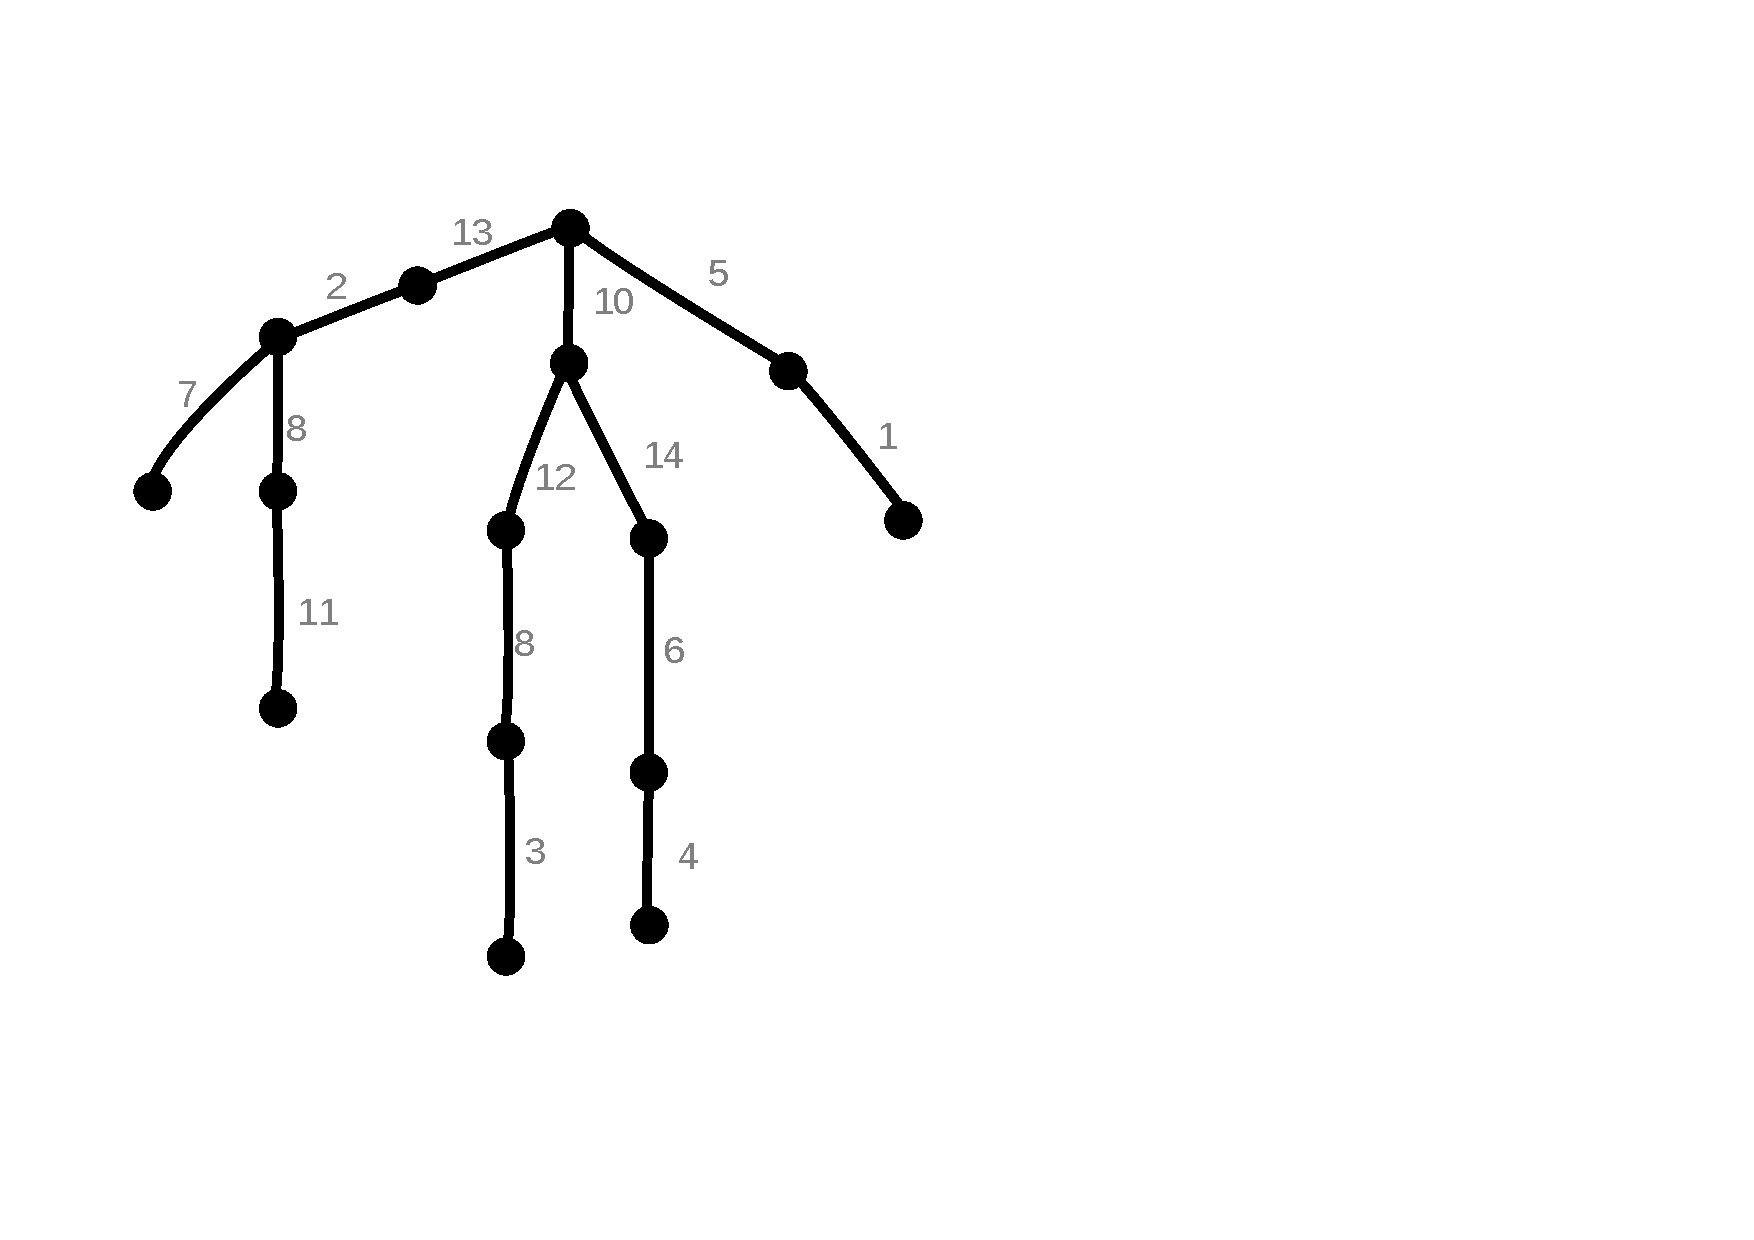
\epsfig{file=exampleplaceholder.pdf, width=.7\linewidth}%
\else
        % TODO
\fi
\caption{EXAMPLE PLACEHOLDER (point out a case II edge in the diagram)}
\label{fig:regmin}
\end{figure}

A path between two regional minima is then a sequence of $n$ edges $e_1 ... e_n$
such that $e_1$ and $e_n$ are the only two regional minima
and for each $ 0 \leq i \le n,\ e_i = (a,b,w_1) , e_{i+1} = (b,c,w_2)$

\noindent An edge is path-maximal if it is the edge with greatest weight along a
 path.
The waterfall algorithm then elides all but those edges that are of maximal weight along some path.

\noindent Claim: An edge is path-maximal iff it is not the minimum edge away fro
m either of its endpoints.



Define a graph as $G = (N,E)$
where $N$ is the set of nodes and $E :: N\times N \times \mathbb{N}$ is the set of weighted edges
that must satisfy the following properties:
\begin{enumerate}

\item Transitivity. $(a,b,k) \in E \iff (b,a,k) \in E$, if there is an
  edge from node a to node b, then there is an edge from node b to
  node a of the same weight.

\item Uniqueness.  $(a,b,k_1) \in E\ and\ (a,b,k_2) \implies k_1 =
  k_2$, there is at most one edge between two nodes.

\item We also require that no two edges are of equal weight,
  \[
  (a_1,b_1,k) \in E\ and\ (a_2,b_2,k) \implies a_1 = a_2\ and\ b_1 =
  b_2
  \] 
  This restriction @@@ provide details.

\end{enumerate}

Define a regional-minimum to be an edge that is surrounded by edges of
greater @@@ weight, i.e.  An edge $e = (a,b,k)$ is a regional minimum iff
$\forall c \in E, l \in \mathbb{N} : (c,b,l) \in E \implies l \geq
k\ and\ (a,c,l) \in E \implies l \geq k $ Equivalently, $e$ is the
edge of smallest weight connoted to nodes $a$ and similarly for node
$b$.



This is illustrated with an example in Figure~\ref{fig:surround}.

\begin{figure}
\centering
\ifpdf
        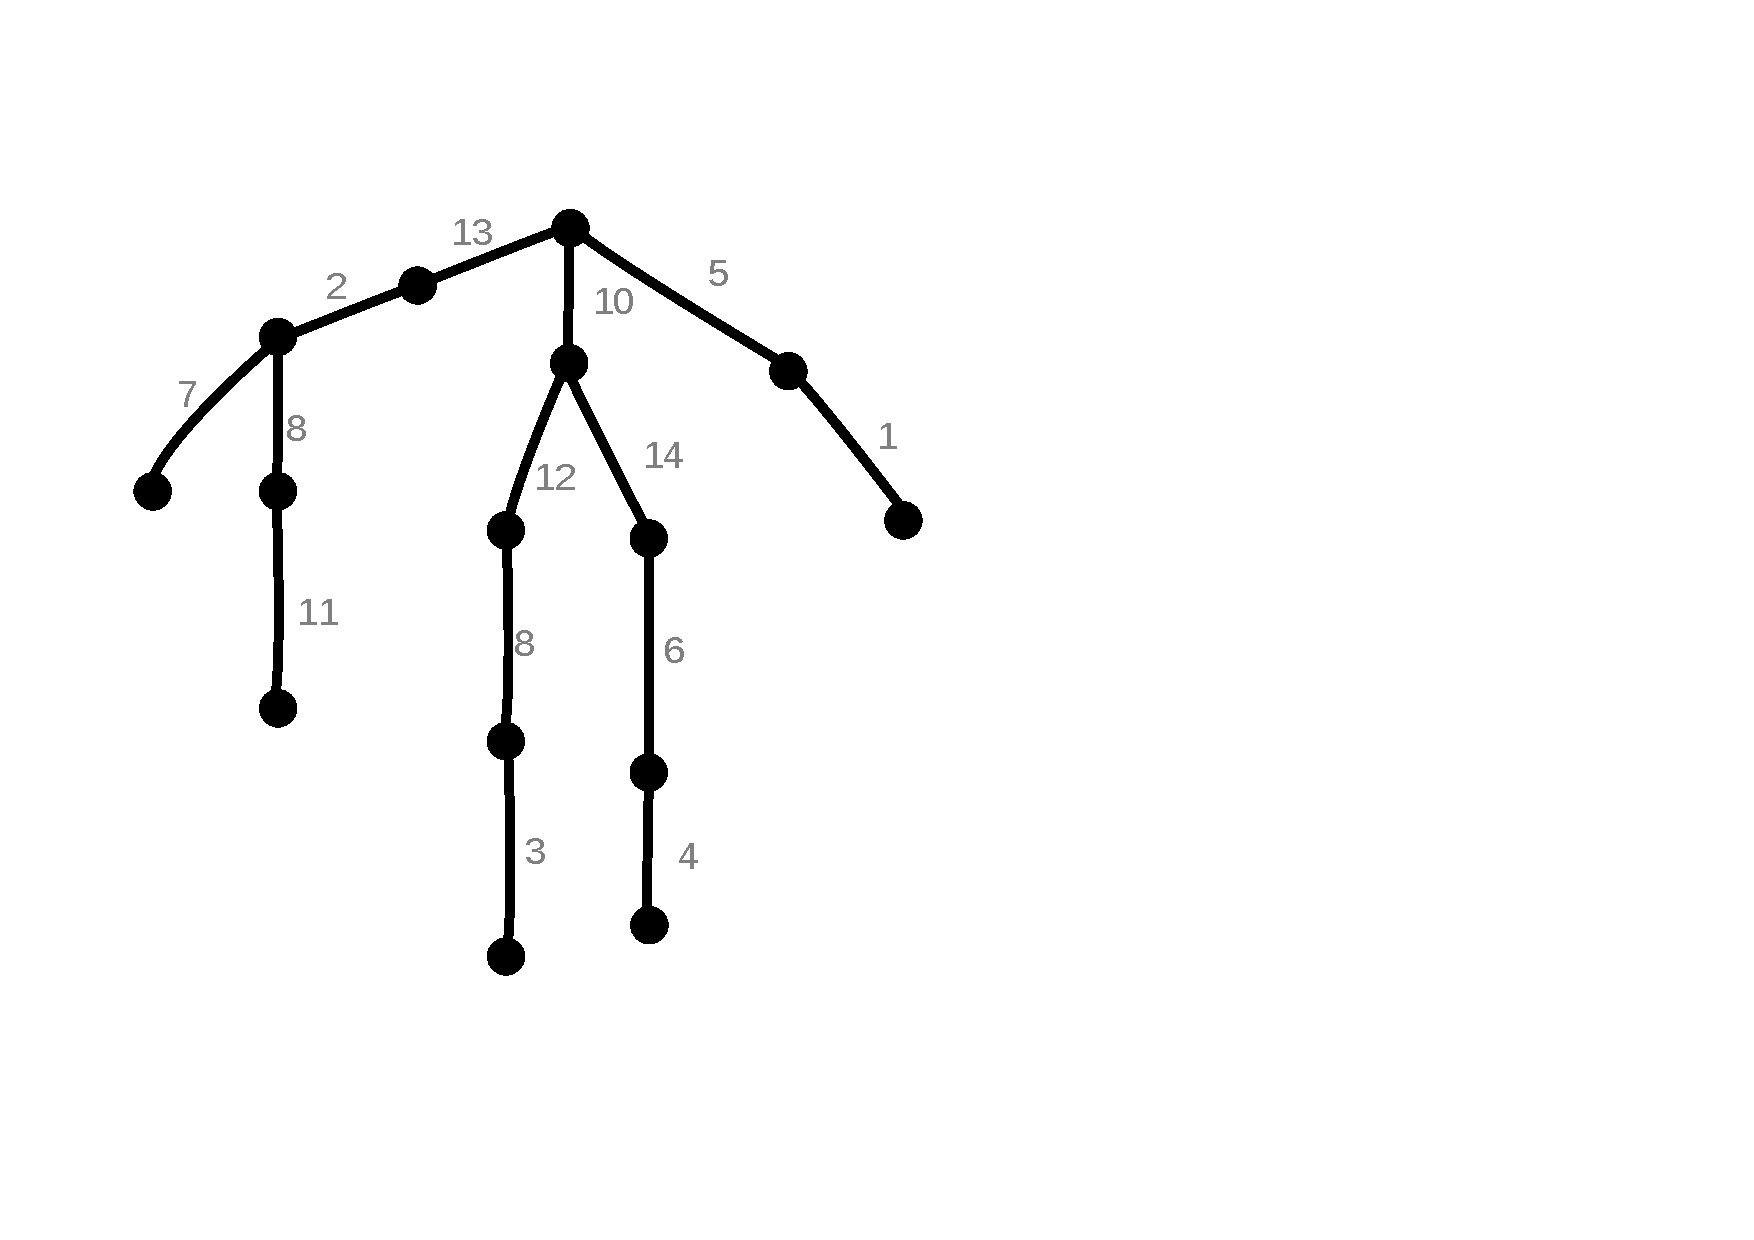
\epsfig{file=exampleplaceholder.pdf, width=.7\linewidth}%
\else
        % TODO
\fi
\caption{EXAMPLE PLACEHOLDER}
\label{fig:surround}
\end{figure}


A path between two regional minima is then a sequence of $n$ edges $e_0 ... e_{n-1}$
such that $e_0$ and $e_n$ are the only two regional minima
and for each $ 0 leq i < n,\ , \exists a,b,c \in N \colon e_i = (a,b,w_1) , e_{i+1} = (b,c,w_2)$

\noindent An edge is path-maximal if it is the edge with greatest weight along a path.
The waterfall algorithm then elides all but those edges that are of maximal weight along some path.

\noindent Claim: An edge is path-maximal iff it is not the minimum edge away from either of its endpoints.

\begin{proof}:

\noindent `$\Rightarrow$'
\indent
  Let $e$ be an edge in the graph and suppose it is path-maximal.
  By definition there exists a sequence of edges $e_0 ... e_{n-1}$
  with $c = e_i$ for some $ 0 \leq i leq n$. Clearly $i \neq 0$ and $i \neq n$ since
  $e_i$ and $e_n$ must be regional minima. Therefore at each end of $c$ there is another edge
  leading from that node with weight smaller than that of $c$, so $c$ is
  not the minimum edge away from either of its endpoints.


\noindent
`$\Leftarrow$'
\indent
  Let $e = (n_1,n_2,w_e)$ be an edge such that it is not the minimum edge away from either of its endpoints.
  Let  $a_0$ be the minimum edge connected to $n_1$ and $b_0$ be the minimum edge connected to $n_2$

  Create a sequence of edges from $n_1$ by always picking the smallest edge from the current vertex until
  you the smallest edge is already in the sequence.
  Do  the same for $n_2$
  Show the endpoints of these sequences are regional minima
  Therefore e is path maximal.
  ....


\end{proof}


(note that there is arbitrary choice about edges of same weight)


\subsection{Plateaux}

Discuss briefly the types of plateaux that can occur and their
influence on the possible results.

Point out that this issue went totally unspecified in the original
algorithm.


\section{Discussion}

\subsection{MST}

generating the MST in grid mode, plus tricks

\subsection{Results}

Lack of gradient image, pre-processing and mosaic display may make the
results look a bit simplistic, but here are some simple examples.


\section{Conclusions}

 - can be done in pure FP style

(When implementing this in an imperative language, the four cases can
 be reduced to just two, on nodes, but then two passes are necessary.)

 - clearer to write/code

 - shorter code and simpler data structures


The main advantage of our approach to the waterfall problem is that
the algorithm uses a single loop to walk the MST and is therefore
simpler to implement. For each iteration, it walks the MST bottom-up
in a single pass and merges regions that belong together. The
waterfall algorithm, thus improved, produces the same layers of
segmented images, combined in a hierarchical structure that can be
processed for feature identification.

A further advantage of our approach is that the algorithm can can be
written in pure functional style. In particular, we have implemented
it in Haskell. For this reason, the memory requirements are not
directly comparable to existing imperative implementations, but we are
about to integrate this new approach into an existing C++ code base.

We are also in the process of constructing a formal proof of
correctness, which we hope to present at a later date. We have tested
both algorithms on a number of small, measurable test cases and found
that they produce the same output. Empirical tests indicate that this
is also true of larger test cases, such as axial slices of CT volumes.

Production of partition forests in this manner is independent of this
application and has many applications outside of the field of medical
imaging.

\subsection{Acknowledgements}

John Fell

Charles Bryant



\bibstyle{plain}

\begin{thebibliography}{99}

\bibitem[Golodetz et al]{golodetz} Stuart Golodetz, Irina Voiculescu
  and Stephen Cameron.  {\em Region Analysis of Abdominal CT Scans
    using Image Partition Forests}. In Proceedings of CSTST
  2008. Pages 432-7. October 2008.

\bibitem[Beucher 1979]{beucher79} S.\ Beucher, C.\ Lantuejoul. {\em
  Use of watersheds in contour detection}. International Workshop on
  image processing, real-time edge and motion detection/estimation,
  Rennes, France. Sept.\ 1979.

\bibitem[Beucher 1994]{beucher94} Serge Beucher. {\em Watershed,
  hierarchical segmentation and waterfall algorithm}. In Mathematical
  Morphology and its Applications to Image Processing, Proc.\ ISMM 94,
  pages 69-76, Fontainebleau, France, 1994. Kluwer Ac.\ Publ.

\bibitem[Marcotegui and Beucher 2005]{marcotegui}{Marcotegui and
  Beucher} Beatriz Marcotegui and Serge Beucher. {\em Fast
  Implementation of Waterfall Based on Graphs}. In {Mathematical
  Morphology: 40 Years On}. Springer Netherlands, 2005.

\end{thebibliography}

\end{document}
